\hypertarget{barcode_8inc}{
\section{include/barcode.inc File Reference}
\label{barcode_8inc}\index{include/barcode.inc@{include/barcode.inc}}
}
Functions for the handling of different barcodes. 

\subsection*{Functions}
\begin{CompactItemize}
\item 
\hyperlink{barcode_8inc_b34ec866d27061573a5fa623bf314fc1}{checkBarcode} (\$barcode, \$type= 'upc')
\item 
\hyperlink{barcode_8inc_e10c37e4f9f9b7c6617a388351a27c99}{getBarcodeInfo} (\$barcode)
\end{CompactItemize}


\subsection{Detailed Description}
Functions for the handling of different barcodes. 

This file currently deals with the handling of barcodes and getting the information associated with them. 

Definition in file \hyperlink{barcode_8inc-source}{barcode.inc}.

\subsection{Function Documentation}
\hypertarget{barcode_8inc_b34ec866d27061573a5fa623bf314fc1}{
\index{barcode.inc@{barcode.inc}!checkBarcode@{checkBarcode}}
\index{checkBarcode@{checkBarcode}!barcode.inc@{barcode.inc}}
\subsubsection{\setlength{\rightskip}{0pt plus 5cm}checkBarcode (\$ {\em barcode}, \$ {\em type} = {\tt 'upc'})}}
\label{barcode_8inc_b34ec866d27061573a5fa623bf314fc1}


Checks to see if a valid, handalable, barcode was entered. \begin{Desc}
\item[Parameters:]
\begin{description}
\item[{\em \$barcode}]The Barcode to be checked \item[{\em \$type}]= The type of barcode, either \char`\"{}upc\char`\"{} or \char`\"{}isbn\char`\"{}. Defaults to what is passed in the HTTP GET information if available, otherwise assumes \char`\"{}upc\char`\"{}. \end{description}
\end{Desc}
\begin{Desc}
\item[Returns:]The type of barcode entered if valid, FALSE if it is not \end{Desc}


Definition at line 20 of file barcode.inc.

References XMLRPC\_\-prepare(), and XMLRPC\_\-request().

\begin{Code}\begin{verbatim}20                                                {
21   if (isset($_GET['type'])) {
22     $type = $_GET['type'];
23   }
24 
25   switch ($type) {
26     case 'upc':
30       $result = XMLRPC_request('dev.upcdatabase.com', '/rpc', 'lookupUPC', array(XMLRPC_prepare($barcode)));
31       if ($result[1] != 'Error: Invalid length') {
32         if (strlen($barcode) == 12) {
33           return 'upca';
34         }
35         else if (strlen($barcode) == 13) {
36           return 'ean13';
37         }
38         else {
39           return FALSE;
40         }
41       }
42       else {
43         return FALSE;
44       }
45       break;
46     case 'isbn':
47       if (strlen($barcode) == 10) {
48         return 'isbn';
49       }
50       else if (strlen($barcode) == 13) {
51         return 'bookland';
52       }
53       else {
54         return FALSE;
55       }
56       break;
57   }
58 }
\end{verbatim}
\end{Code}




Here is the call graph for this function:\nopagebreak
\begin{figure}[H]
\begin{center}
\leavevmode
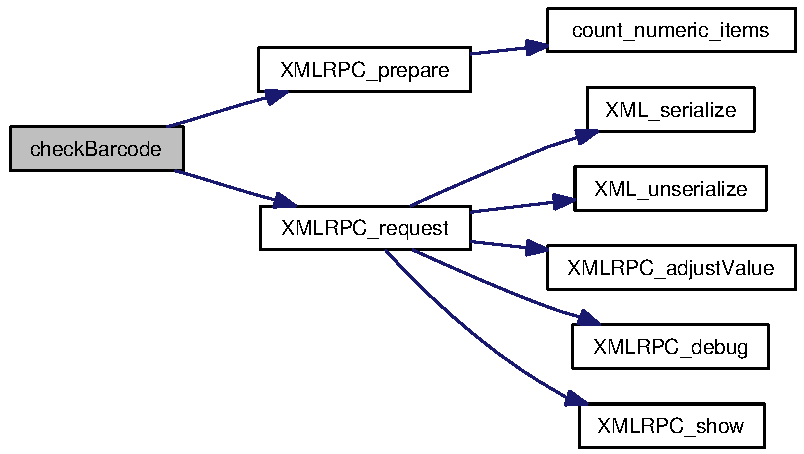
\includegraphics[width=211pt]{barcode_8inc_b34ec866d27061573a5fa623bf314fc1_cgraph}
\end{center}
\end{figure}
\hypertarget{barcode_8inc_e10c37e4f9f9b7c6617a388351a27c99}{
\index{barcode.inc@{barcode.inc}!getBarcodeInfo@{getBarcodeInfo}}
\index{getBarcodeInfo@{getBarcodeInfo}!barcode.inc@{barcode.inc}}
\subsubsection{\setlength{\rightskip}{0pt plus 5cm}getBarcodeInfo (\$ {\em barcode})}}
\label{barcode_8inc_e10c37e4f9f9b7c6617a388351a27c99}


Output Barcode Info \begin{Desc}
\item[Parameters:]
\begin{description}
\item[{\em \$barcode}]The barcode to lookup \end{description}
\end{Desc}
\begin{Desc}
\item[Returns:]HTML code to create the info area \end{Desc}
\begin{Desc}
\item[See also:]\hyperlink{barcode_8inc_b34ec866d27061573a5fa623bf314fc1}{checkBarcode} \end{Desc}


Definition at line 66 of file barcode.inc.

References getImages(), parseXML(), XMLRPC\_\-prepare(), and XMLRPC\_\-request().

\begin{Code}\begin{verbatim}66                                   {
67   switch ($_GET['type']) {
68     case 'upc':
72       $output = '';
73       $output .= '<div id="upc">';
74       $output .= '<img src="upcimg.php?upc=' . $barcode . '" />';
75       $output .= '</div>';
76 
80       $result = XMLRPC_request('dev.upcdatabase.com', '/rpc', 'lookupUPC', array(XMLRPC_prepare($barcode)));
81       $output .= getImages($result[1]['description']);
82       if ($result[1]['found']) {
83         extract($result[1], EXTR_PREFIX_ALL, 'barcode');
84         $output .= <<<_HTML
85         <div id="info">
86           <table align="center">
87             <tr>
88               <td class="title">Country</td>
89               <td>$barcode_issuerCountry</td>
90             </tr>
91             <tr>
92               <td class="title">Description</td>
93               <td>$barcode_description</td>
94             </tr>
95             <tr>
96               <td class="title">Size</td>
97               <td>$barcode_size</td>
98             </tr>
99           </table>
100           <a href="http://www.upcdatabase.com/editform.asp?upc=$barcode">Modify this entry</a>
101           <a href="http://www.upcdatabase.com/deleteform.asp?upc=$barcode">Delete this entry</a>
102         </div>
103 _HTML;
104       }
105       else {
106         $output .= 'Product Not Found!<br />';
107         $output .= '<a href="http://www.upcdatabase.com/addform.asp?upc=' . $barcode . '">Add this item to the database</a>';
108       }
109       break;
110 
111     case 'isbn':
115       $xml = parseXML('http://isbndb.com/api/books.xml?access_key=' . ISBNKEY . '&index1=isbn&results=texts&value1=' . $barcode);
116 //       var_dump($xml);
117 
118       // Sometimes, the long title is non-existant, so fall back onto the short title
119       if (strlen($xml->BookList->BookData->TitleLong) != 0) {
123         $title = $xml->BookList->BookData->TitleLong;
124       }
125       else {
129         $title = $xml->BookList->BookData->Title;
130       }
134       $author = $xml->BookList->BookData->AuthorsText;
138       $publisher = $xml->BookList->BookData->PublisherText;
142       $summary = $xml->BookList->BookData->Summary;
146       $isbn = $xml->BookList->BookData['isbn'];
147 
151       $output = '';
152       $output .= '<div id="upc">';
153       $output .= '<img src="upcimg.php?upc=' . $barcode . '" />';
154       $output .= '</div>';
155       $output .= getImages($title, 'book');
156       $output .= <<<_HTML
157       <div id="info">
158         <table align="center">
159           <tr>
160             <td class="title">Title</td>
161             <td>$title</td>
162           </tr>
163           <tr>
164             <td class="title">Author</td>
165             <td>$author</td>
166           </tr>
167           <tr>
168             <td class="title">Publisher</td>
169             <td>$publisher</td>
170           </tr>
171           <tr>
172             <td colspan="2">$summary</td>
173           </tr>
174           <tr>
175             <td class="title">Buy</td>
176             <td>
177               <!-- Amazon.com uses the ISBN-10 code, so send it that -->
178               <a href="http://www.amazon.com/exec/obidos/ASIN/$isbn/">Amazon.com</a><br />
179               <!-- Everyone else uses the ISBN-13 code, so send them that -->
180               <a href="http://search.barnesandnoble.com/booksearch/isbninquiry.asp?ean=$barcode">Barnes & Noble</a><br />
181               <a href="http://www.booksamillion.com/ncom/books?type=isbn&find=$barcode">Books-A-Million</a><br />
182               <a href="http://www.google.com/products?q=$barcode">Google Product Search</a>
183             </td>
184           </tr>
185         </table>
186       </div>
187 _HTML;
188       break;
189   }
190 
191   return $output;
192 }\end{verbatim}
\end{Code}




Here is the call graph for this function:\nopagebreak
\begin{figure}[H]
\begin{center}
\leavevmode
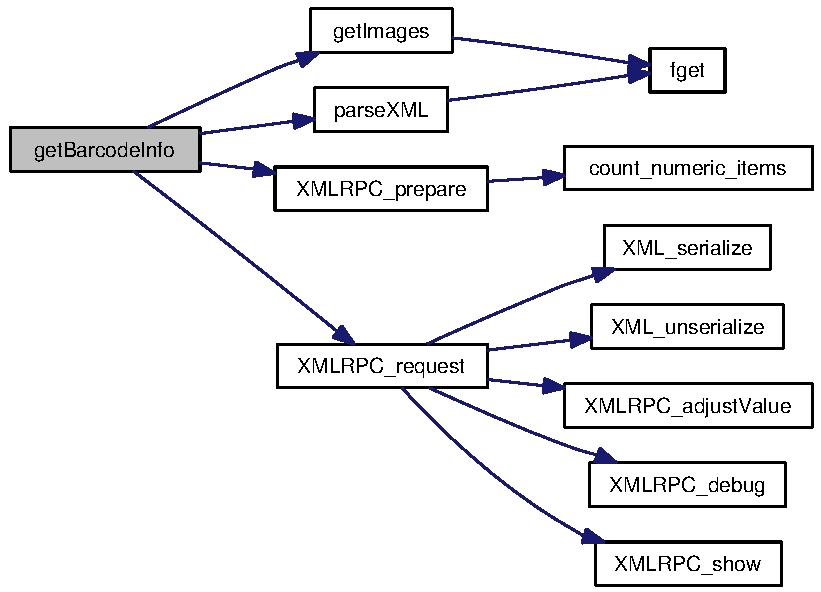
\includegraphics[width=215pt]{barcode_8inc_e10c37e4f9f9b7c6617a388351a27c99_cgraph}
\end{center}
\end{figure}
